\documentclass{beamer}
\usetheme{metropolis}
\usepackage{listings}
\usepackage{xcolor}

\title{Object Oriented Programming}
\author{Jannusch Bigge}
\date{05.12.2023}

\begin{document}
\begin{frame}
    \titlepage
\end{frame}

\section{Objetc Oriented Programming}

\begin{frame}{Object Oriented Programming}
    \begin{itemize}
        \item Python is an object oriented programming language
        \item Everything is an object
        \item Objects have attributes and methods
        \item Attributes are variables
        \item Methods are functions
    \end{itemize}
\end{frame}

\begin{frame}[fragile]{Object Oriented Programming}
    What is an object?\\\pause
    \only<2->{\begin{itemize}
        \item An instance of a class
    \end{itemize}
    }\pause
    What is a class?
    \only<3->{
        \begin{itemize}
        \item A blueprint for an object
    \end{itemize}
    }\pause
\begin{alertblock}{You can create multiple objects from one class!}
    
\end{alertblock}
\end{frame}

\begin{frame}{Example - OOP}
We have a blueprint for a car.\\
And wie create three cars from this blueprint.\pause
    \begin{center}
        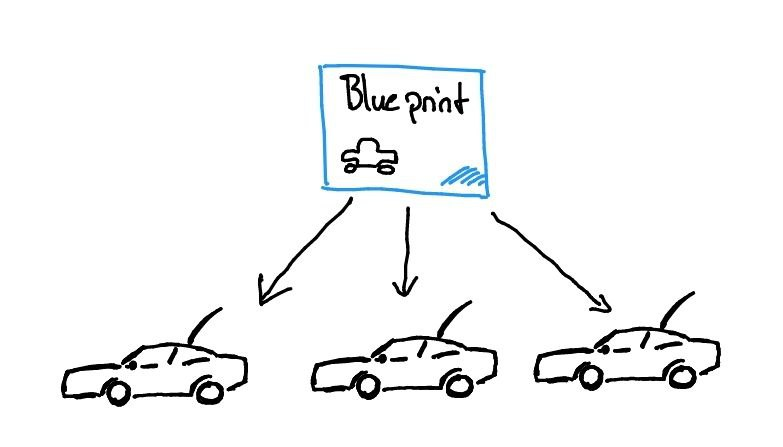
\includegraphics[width=0.7\textwidth]{figures/nomal.jpg}
    \end{center}
\end{frame}

\begin{frame}[fragile]{Example - OOP}
    \begin{lstlisting}[language=Python]
    class Car:
        def __init__(self) -> None:
            print("Created a new car")
        
    car1 = Car()
    car2 = Car()
    car3 = Car()

    \end{lstlisting}

\end{frame}


\begin{frame}{OOP - Attributes}
    \begin{itemize}
        \item Attributes are variables
        \item They are defined in the \texttt{\_\_init\_\_} method
        \item They are accessed with \texttt{self}
    \end{itemize}
    \begin{center}
        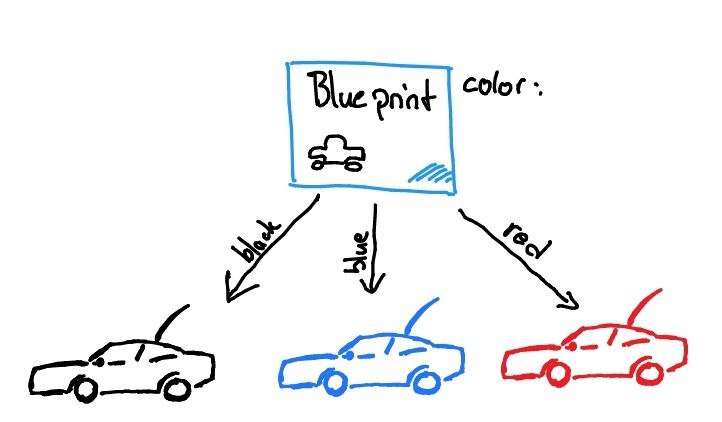
\includegraphics[width=0.7\textwidth]{figures/attribut_color.jpg}
    \end{center}

\end{frame}

\begin{frame}[fragile]{Example - OOP}
    \begin{lstlisting}[language=Python]
    class Car:
        def __init__(self, color: str) -> None:
            print("Created a new car")
            self.color = color
        
    car1 = Car("black")
    car2 = Car("blue")
    car3 = Car("red")

    \end{lstlisting}
       
\end{frame}

\begin{frame}{OOP - Methods}
    
    \begin{itemize}
        \item Methods are functions of the object
        \item They are defined in the class
        \item Accessing attributes with \texttt{getter and setter}
        \item Called by referencing the object
    \end{itemize}
    To get the color of the car we need a getter method.

\end{frame}

\begin{frame}[fragile]{Example - OOP}
    \begin{lstlisting}[language=Python]
    class Car:
        def __init__(self, color: str) -> None:
            print("Created a new car")
            self.color = color

        def get_color(self) -> str:
            return self.color
        
    car1 = Car("black")
    color = car1.get_color()
    print(f"The car is: {color}")
    >>> The car is: black
    \end{lstlisting}
       
\end{frame}

\begin{frame}{OOP - Inheritance}
    We are interested in different cars.\\\pause
    \only<2>{\begin{center}
        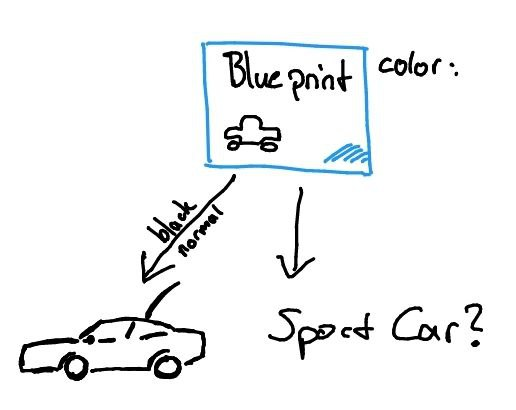
\includegraphics[width=0.7\textwidth]{figures/how_different_type.jpg}
    \end{center}
    }
    \only<3,5-6>{Solutions:
        \begin{itemize}
            \item<3, 5-6> Create a attribute "type"
            \item<6> Create a new class "sort car"
        \end{itemize}
    }
    \only<4>{\begin{center}
        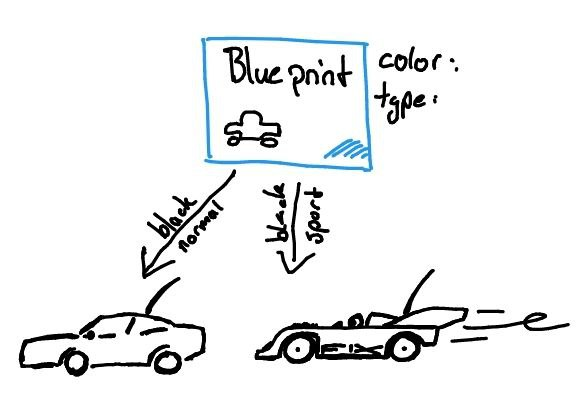
\includegraphics[width=0.7\textwidth]{figures/attribute_type.jpg}
    \end{center}
    }
    \only<5>{
                \textbf{But what if we want to add a attribute only for one type?}
                e.g. race license 
    }
    \only<7>{
        Create a new class "sport car" that inherits from "car"
        \begin{center}
            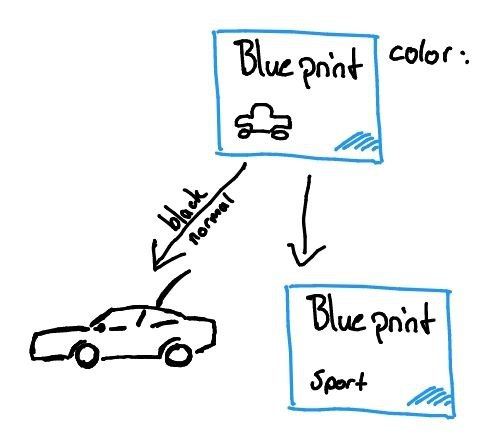
\includegraphics[width=0.7\textwidth]{figures/inheritance.jpg}
        \end{center}
    }

\end{frame}

\begin{frame}{OOP - Inheritance}
    \begin{itemize}
        \item Inheritance is a way to create a new class from an existing class
        \item The new class is called child class
        \item The existing class is called parent class
        \item The child class inherits the attributes and methods of the parent class
        \item The child class can overwrite and add attributes and methods of the parent class
    \end{itemize}
\end{frame}

\begin{frame}{OOP - Inheritance}
    \begin{center}
        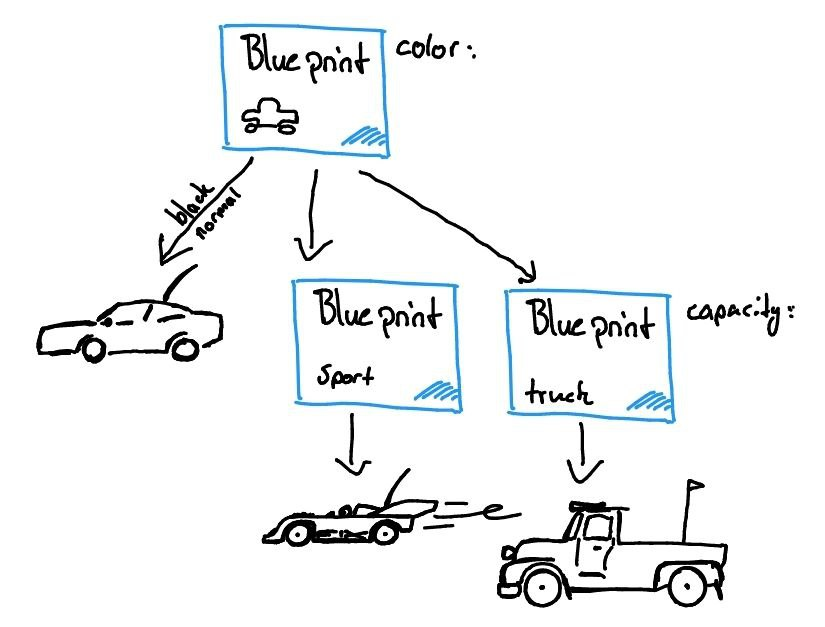
\includegraphics[width=0.9\textwidth]{figures/full_inheritance.jpg}
    \end{center}
\end{frame}

\begin{frame}[fragile]{Example - OOP}
    \begin{lstlisting}[language=Python]
class Car:
    def __init__(self, color: str) -> None:
        print("Created a new car")
        self.color = color

    def get_color(self) -> str:
        return self.color
        
class SportCar(Car):
    def __init__(self, color: str, license: bool):
        super().__init__(color)
        self.license = license
        
car1 = Car("black")
car2 = SportCar("blue", True)
    \end{lstlisting}
\end{frame}

\section{Magic Methods}
\begin{frame}{Magic Methods}
    \begin{itemize}
        \item Magic methods are special methods that are called by special syntax
        \item They are used to implement operator overloading
        \item They are defined with two underscores before and after the name
        \item Normally they are called by the interpreter and only implicitly by the user
    \end{itemize}
    We already used the \texttt{\_\_init\_\_} method.

\end{frame}

\begin{frame}[fragile]{Magic Methods}
    \begin{lstlisting}[language=Python]
        def __gt__(self, other):
            return self.hp > other.hp
    \end{lstlisting}
        
    \end{frame}


\section{List Comprehension}

\begin{frame}{List Comprehensions}
    \begin{itemize}
        \item List comprehensions are a way to create lists
        \item They are more compact than for loops
        \item They are faster than for loops
        \item They are more readable than for loops (sometimes)
    \end{itemize}
\end{frame}

\begin{frame}[fragile]{List Comprehensions}

    newlist = [expression \textbf{for} item \textbf{in} iterable \textbf{if} condition == True]
    \begin{lstlisting}[language=Python]
    # Create a list with the numbers from 0 to 9
    #old way
    numbers = []
    for i in range(10):
        numbers.append(i)#

    # with list comprehensions
    numbers = [i for i in range(10)]
    odd = [i for i in range(10) if i % 2 == 1]
    \end{lstlisting}
\end{frame}

\section{Task}


\end{document}

